% useful commands
% \medskip , \smallskip, \noindent, \vspace{0.2in}
% \sc (all caps)
%




\documentclass[11pt]{article}   % For Latex2e
\usepackage{amssymb,amscd,latexsym}   % For Latex2e
\usepackage{amsmath}
\usepackage{amsthm}
\usepackage{epsfig}
\usepackage{enumerate}
\usepackage{listings}
\usepackage{moreverb}
\usepackage{amssymb} % for \smallsetminus

\usepackage{mathtools} % allows you to use \boxed or \Aboxed
\usepackage{mhchem}
%%%%%%%%%%
%\topmargin=-0.5cm
%\marginparwidth=2cm
\textwidth=6.3in
\textheight=22cm
\hoffset=-1.8cm
\voffset=-1.3cm
%%%%%%%%%%%%%%%%%%%
\def\vdotfill{
\vbox to 2em
{\cleaders\hbox{.}\vfill}}
%------------------------

\usepackage{listings}
\usepackage{color}

\definecolor{dkgreen}{rgb}{0,0.6,0}
\definecolor{gray}{rgb}{0.5,0.5,0.5}
\definecolor{mauve}{rgb}{0.58,0,0.82}
\newcommand{\dcomment}[1]{\textcolor{red}{#1}}
\lstset{frame=, %tb
  language=Java,
  aboveskip=1mm,
  belowskip=1mm,
  showstringspaces=false,
  columns=flexible,
  basicstyle={\small\ttfamily},
  numbers=none,
%  numberstyle=\tiny\color{gray},
%  keywordstyle=\color{blue},
  commentstyle=\color{dkgreen},
  escapeinside={\%*}{*)},
  stringstyle=\color{mauve},
  breaklines=true,
  breakatwhitespace=true,
  tabsize=3
}

\newtheorem{Theorem}{Theorem}[section]
\newtheorem{Lemma}[Theorem]{Lemma}
\newtheorem{Corollary}[Theorem]{Corollary}
\newtheorem{Proposition}[Theorem]{Proposition}
\newtheorem{Remark}[Theorem]{Remark}
\newtheorem{Example}[Theorem]{Example}
\newtheorem{Conjecture}[Theorem]{Conjecture}
\newtheorem{Definition}[Theorem]{Definition}
\newtheorem{Question}[Theorem]{Question}
%%%%%%%%%%%%%%%%%%%%%%%%%%
\newcommand{\rar}{\rightarrow}
\newcommand{\lar}{\longrightarrow}
\newcommand{\llar}{-\kern-5pt-\kern-5pt\longrightarrow}
\newcommand{\surjects}{\twoheadrightarrow}
\newcommand{\injects}{\hookrightarrow}
\newcommand{\Fiber}{{\cal F}}

\renewcommand{\phi}{\varphi}
\newcommand{\demo}{{\sc Proof. }}
\renewcommand{\proof}{\demo}
%\newcommand{\demo}{\noindent{\sc Proof. }}
%\newcommand{\square}{\mathchoice\sqr64\sqr64\sqr{4}3\sqr{3}3}
%\newcommand{\qed}{\hspace*{\fill} $\square$}
%\newcommand{\QED}{\hbox{\qed}}





\newcommand{\restr}{{\kern-1pt\restriction\kern-1pt}}




\begin{document}

\begin{center}

\vspace{3in}
{\Huge{\bf\sc Evolution Three}}\\
\vspace{.1in}
{\small\sc ECE 458}


\vspace{0.3in}



{\large\sc Parker Hegstrom} {\large (eph4)} \\
{\large\sc Peter Yom} {\large (pky3)} \\
{\large\sc Wayne You} {\large (wxy)} \\
{\large\sc Brandon Chao} {\large (bc105)} \\


\end{center}


\vspace{0.2in}

\begin{abstract}
In this evolution, we added two new features to our shared calendar web application. Specifically, a user can now create Slot Sign Up events, which allow other users to ``sign up" for an appointment. The second feature is more a service as it allows the user to determine who has event conflicts given certain time frames. In addition to these new features, some major refactoring was done and will be further explained in the following document.
\end{abstract}

\tableofcontents


\pagebreak


\section{Overall Design}

The overarching design principle we wanted to achieve was modularity. In doing so, we believed we would be able to work separately (with occasional meetings to work through minor problems with the API) and refactor without the worry of breaking another \dcomment{member's} code. Figure \ref{design} below shows a high level diagram of how we decided to design our calendar web application.

\begin{figure}[htb]
\centering
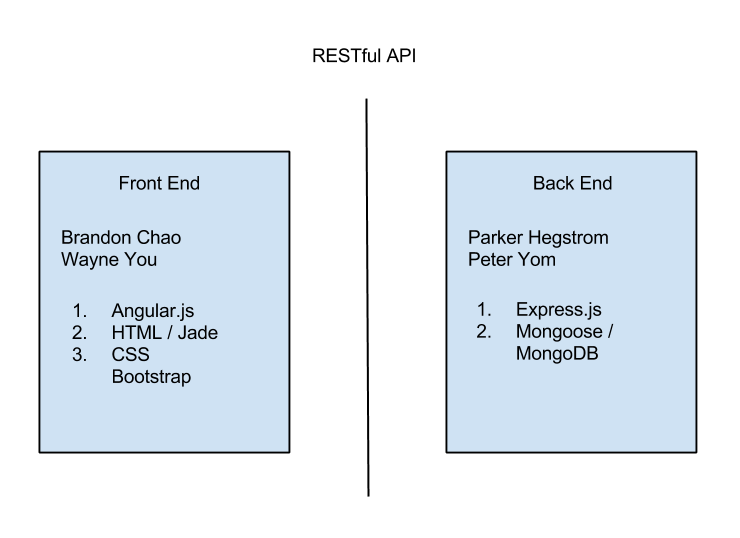
\includegraphics[width=.5\textwidth]{DesignDiagram.png}
\caption{Diagram of our Large Scale Design}
\label{design}
\end{figure}

\noindent Essentially, our back end team provides an exhaustive RESTful API service to our front end. As we received the new requirements for evolution two, the benefits of our modular design came to light as we met to discuss both the refactorings from evolution one that needed to be done and the edits to each modules system design in order to account for the added calendar functionality--event requests and persistent until done events.\\

\noindent At the beginning of evolution three, our group spent four days simply refactoring and making large design change decisions.  The back-end did undergo one major change as we now handle repeated events differently. The front-end also made a fundamental change with how Angular controllers are implemented. These will be further discussed in the following section.\dcomment{(In 2.3 you only mention the repeating events part. Was that really all 4 days?  Were these other refactorings not indicative of weaknesses that you should discuss there?) }\\

\noindent The following sections further discuss design choices and implications of those design choices for both our front end and back end teams. \\

\section{Back End Design and Analysis}
\subsection{New Features and Developments}
The two new features as well as other design developments are discussed below:
\dcomment{(Really no need for this subsection if you aren't going to say anything here.  Just
make the subsubsections into subsections.)}
\subsubsection{Slot Sign Up Events}
To implement the slot sign up feature, we created an entirely new structure in the database. This structure, \texttt{SlotSignUp.js}, allowed us to develop without the fear of breaking something already created in the first two evolutions of the project. To handle the dynamic nature of the \texttt{SlotSignUp}, we used the composition design pattern. More specifically, a \texttt{SlotSignUp} is composed of individual \texttt{Slots}, which can be created and associated with any user that signs up for a specific \texttt{Slot}. Initially, though, the \texttt{SlotSignUp} is composed of free blocks of minimum sign up length. As people sign up for slots, the \texttt{Slot} objects are created and tied to that user. This information is stored in the \texttt{attendees} property of the \texttt{SlotSignUp}. \\

\noindent A user must be able to determine the status of the sign up slot (list attendees, what blocks they've signed up for, what free time is left, etc.), and we wanted to make this information as easy as possible to display and edit for the front end. Hence, we stored an attendee's \texttt{email} with his/her slots. This allowed for immediate access to client-ready, displayable information and removed the need for the client to issue additional database queries. Before, the client would have been given a list of user ids and would have had to query the DB with those ids, presenting un-needed latencies to the end user of our application.\\

\noindent Lastly, we wanted the slot sign up to be easily modified or extended in the future, thus was the impetus for using the composition pattern. The \texttt{Slot} was extracted into its own model file and is therefore independent of the \texttt{SlotSignUp}. Say, for example, we wanted to add Alerts to our individual Slots. This would be as easy as creating a new \texttt{Alert} property in \texttt{Slot.js}.

\subsubsection{Find Free Times}
\noindent Find free times did not require any database changes, nor did it require any new models to be created. This requirement was solely algorithm driven and the control for this feature can be found in \texttt{freeTimeRoutes.js}. \\

\noindent There is one route in \texttt{freeTimeRoutes.js}: \texttt{PUT /ftr/findConflicts}.  The goal of this route is to accept users, usergroups, and a list of time slots, and return a comprehensive 'conflict summary'. \\

\noindent First, an array of available events is created from each passed in user.  This array contains only events that the logged in user  has view, modify, or view-busy access to from the list of passed in users and user groups.  The array of all events is sorted by \texttt{start} time. On the other hand, the list of time slots is sorted by \texttt{end} time.  We then developed an algorithm to compare the array of events with the array of time slots in $O(n+m)$ time with $m$=number of events and $n$=number of time slots.  In the conflict summary, each time slot has an array of events which conflict (aka have times that interfere with the start and/or end times of the time slot). \\

\noindent In the conflict summary, each time slot also has an array of free times between the start and end times for the time slot. This is determined with the 'slotSize' in mind. \\

\noindent We designed the conflict summary to be as complex and detailed as possible to minimize the number of calculations needed to be done by the front end.

\subsubsection{New Implementation for Repeated Events}
Before, our repeated events were somewhat fake and display driven. We would have one real event in the data base and simply display the event in the future if there was a repeat. We decided we wanted a more powerful approach, one that allowed for repeated events to behave similarly (deleting all at once, sharing same properties) but also behave independently. This new implementation also allowed our code for Find Free Times to run and handle the repeats properly without any additional modification.\\

\noindent To implement this new design, we created a new structure, the \texttt{RepeatChain}. The purpose of this structure was to keep track of all events that were created as a repeat chain, allowing us to edit individual events in the chain as well as delete all repeated events the same time.

\subsubsection{Async.js}
One difficult\dcomment{y} we've mentioned many times in our discussions and presentations has been the asynchronous nature of javascript. In this evolution, we further implemented a new node module: \texttt{asyn.js}. Under the hood this module works with promises, but this api allowed us \dcomment{to} control asynchronous dependencies. After witnessing the power of this module, we were able to clean up the call back hell situations we got ourselves into in the past.

\subsubsection{Schema Methods}
Before this evolution, we never used Mongoose Schema methods which \dcomment{left} our route files cluttered and at times difficult to read. Schema methods allowed us to extract Schema specific behavior and treat our Schemas like classes with an api. For example, we have a \texttt{User} schema. Adding a schema method allowed us to call functions on a \texttt{User} like \texttt{User.convertToEmail()}. Extracting schema methods severely cut back on our repeated code throughout the project. For a working example, see \texttt{./models/User.js}.

\subsection{Benefits of Our Previous Design}
The major benefit of our previous design was its modularity and composition-driven nature. The modularity allowed for easy addition of new features and simultaneous development by all of our team members. It also allowed for easy and testable code as well, because we could test single files or single methods that composed the entire module.\\

\noindent The composition-driven nature of our design proved to be the most powerful thing we've done thus far. That is, we were able to add new features or extend the functionality of previously working code in extremely easy manner, all the while having these changes to database model files persisted throughout the entire database. For example, this evolution required a User to be able to keep track of slots he/she had signed up for or sign up events he/she had created. This was easily done by adding a new property to the Schema Model that ``pointed" to the actual \texttt{Slot} or \texttt{SlotSignUp} objects in the database.

\subsection{Drawbacks of Our Previous Design}
The way we initially design\dcomment{ed} and implemented repeated events proved to be extremely limiting with the new requirements of evolution three. As mentioned before, repeated events used to be simply display-driven, meaning that there was really only one event stored in the data base.\\

\noindent This shortfall was changed such that all repeated events are now actual events in the database.

\dcomment{This subsection is rather short.  If you spent 4 days refactoring your code, it seems
  like you should have had a \emph{lot} to say here.}

\section{Front End Design and Analysis}

\subsection{New Features and Developments}

\subsubsection{Find Free Times}
Find free times was implemented in the frontend by simply creating new modals to allow users to submit the relevant data, view the resulting conflict summary, and create the event and easily send invite requests. These modals were created relatively easily since they are very modular in their design. However, the difficult part was sharing the data between the modals and calling functions across controllers. We achieved this by using Angular services which we will discuss in more detail below. In the first modal, users are able to choose users that they want to find free times for, the size of the block of time to find, and a list of time slots to consider. We also allow users to find free times over recurring weeks. This data is then sent to the backend which returns an object that we use to populate our next modal - the conflict summary. The conflict summary modal is located in a separate controller with the returned object being shared between the two with an Angular service. While viewing the conflict summary, users are then able to choose a suggested open time and create an event at that time. When users create an event out of a conflict summary, they now have the option of inviting everyone in the conflict summary immediately after creating the event. While implementing this, I ran into asynchronous problems which I address in my individual portion below. From here, event creation and user invites function as they did before.

\subsubsection{Slot Sign Ups}
Slot sign-ups were implemented using previous standards of creating a modal for each form and display. The user is able to create a slot-sign up event and designate any number of user groups and users to be associated. They may also add in any number of times so long as the times are multiples of the minimum time. Most of the work here was input validation since the method of adding and removing data for http transfer was already established. For attendee sign-ups, some additional work was needed to allow for sign-up times larger than a single slot that only counted for a single sign-up. This was fixed by allowing a user to create a block of time from a set of option inputs and eventually send a sign-up request to the database. The user is then able to see what times they are signed up for. Unfortunately, the owner of the sign-up event cannot see what the attendees have signed up for. This seems to be a problem with Jade, angular templating within the same file, and angular repeat. There is a nested loop required for displaying all of a user's time slots, but ng-repeat is unable to access the data from the outer loop iteration while within the template.

\subsubsection{Angular Services}

Angular services use dependency injection to allow you to share code between your application. Services are singletons and thus are able to be accessed by all components that are dependent on that service. While previously we had all of our frontend code in two major controllers, by using services we were able to break these up into several smaller controllers and share the relevant scope variables in the service. This allowed more modularity and broke our files into smaller and easier to read parts. This major change has also allowed us to do things that we couldn't before such as open multiple modals in the same portion of our app. Previously this was a challenge because we could not use the same controller to control each modal and define the modal multiple times. However, with services we have been able to create new modal controllers for each modal and just share the relevant variables in the service.

\subsection{Benefits of Our Previous Design}

The inherent modularity of modals made it easy to implement new features on the frontend. We merely had to create a new modal controller and then call the backend HTTP routes out of that. Using Angular's services, we could also share data between these controllers as we needed.

\subsection{Drawbacks of Our Previous Design}

Angular scopes continue to create some problems when trying to debug and circumvent data passing, but the addition of using a service passed around the modals is reducing the effect of the problem. However, the continued increase in the size of our main jade template is becoming problematic. We may need to request the back-end to give us an all-purpose route to get Jade templates rendered individually for modal templates. This would allow us a fix for some of the odd Angular/Jade interactions that are causing unnecessary issues.

\section{Individual Portion}
\subsection*{Parker}

\begin{enumerate} [a)]
\item  {\bf Designing and Conducting Experiments}
\begin{enumerate} [$\cdot$]
\item A problem we were having dealt with the data type of a documents \texttt{\_id} value. This \texttt{\_id} value \dcomment{is } assigned to each document in mongo db. Sometimes we were getting a \texttt{string} and other times the type was \texttt{object}. The experiment was simple. Create a document in the data base and access the \texttt{\_id} property by using various methods. Specifically, I would access it using either \texttt{user.id} or \texttt{user.\_id} and printing out the \texttt{typeof}. Viewing the results yielded the conclusion that \texttt{.id} returns type \texttt{string}.
\end{enumerate}
\item  {\bf Analyzing and Interpreting Data}
\begin{enumerate} [$\cdot$]
\item I think my previous answer also works for this bullet as well. How did I discover that we had a typing problem with the document \texttt{\_.id}? I had noticed weird error messages in the console, analyzing the console to pinpoint where the problem was coming from exactly. Then, after inserting print out statements, I began to study the \texttt{typeof} return value to determine what the end problem was. 
\end{enumerate}
\item {\bf Designing System Components}
\begin{enumerate} [$\cdot$]
\item As mentioned earlier in this document, the way we previously implemented repeated events was not ideal. So, I designed the new repeated events system. I wanted to make the repeated events act as one in some ways, but in other ways be able to act independently. To do this, I made it such that all repeated events are created in the database. They are of the same type as normal events. However, I did create a new data type in the database, the \texttt{RepeatChain}. When an event was created with repeats, a \texttt{RepeatChain} will be created such that the system always knows what events were created by a repeat. This allows for easy deletion or editing of all of the events at a time.
\end{enumerate}
\item {\bf Dealing with Realistic Constraints}
\begin{enumerate} [$\cdot$]
\item One constraint we found was that it was very difficult to create a mongoose schema with JSON object as property value. For example, \dcomment{the} property \texttt{attendees} was composed of an array of JSON objects. For some reason, mongodb / mongoose could not handle the editing of such JSON objects and save them properly. Hence, we had to devise our own way to edit the JSON objects to get around this constraint. The solution: set the property to null, and recreate the JSON object every time rather than try and edit the JSON object individually while still a part of the mongoose document.
\end{enumerate}
\item  {\bf Teamwork and Team Member Interaction}
\begin{enumerate} [$\cdot$]
\item For the most part, everything went very well. All member contributed equally. Specifically, Peter and I met often to discuss progress on our individual work and to discuss what the next design decisions would be. There were some times, though, when there was a lack in communication between the front end and back end which led to some difficult problems down the road.
\end{enumerate}
\end{enumerate}

\subsection*{Peter}

\begin{enumerate} [a)]
\item  {\bf Designing and Conducting Experiments}
\begin{enumerate} [$\cdot$]
\item While developing the algorithms to find conflicting times or slot sign up free times, I would write out simple test code with the simple javascript test tools on \texttt{w3schools.com}.  Javascript Date objects can be compared and modified like simple numbers, as they are essentially large millisecond values, so I tested my algorithms with simple numbers to save time.  After I was satisfied with my tests, I created simple test routes and tested them with PostMan with more realistic values.
\end{enumerate}
\item  {\bf Analyzing and Interpreting Data}
\begin{enumerate} [$\cdot$]
\item We ran into several bugs last minute, and at one point I had to analyze and interpret a million console logs.  I inserted console logs throughout freeTimeRoutes while debugging an issue and eventually found where errors were.
\end{enumerate}
\item {\bf Designing System Components}
\begin{enumerate} [$\cdot$]
\item I designed the creation of the conflictSummary, the merge and compare algorithm to find conflicting events and free times, the slot sign up creation, signing up, and canceling of slots.  I designed the structure of the conflictSummary object to return to the front end.  It is essentially a map with time slots as keys and conflicting events and free times as values.  This makes it very easy for the front end to display conflict data per time slot. Compared to previous evolutions, this evolution was less about creating new structures and more about developing algorithms to process information.  For example, I wrote the algorithm to compare events with time slots to find conflicting events.  I sorted the events by start date and the time slots by end date. Then I had a pointer for each array that would increment accordingly.
\end{enumerate}
\item {\bf Dealing with Realistic Constraints}
\begin{enumerate} [$\cdot$]
\item Javascript's asynchronous nature made development incredibly frustrating at times. At times, we needed functions to be called in a specific order but certain functions, namely anything dealing with calls to the database through Mongoose, would take too long and would complete when it was too late.  Parker and I found the answer to our problems with the async library and the waterfall function.  Waterfall takes in an array of functions and completes the functions in order one after another. This allowed us to have much more control over how our code works.
\end{enumerate}
\item  {\bf Teamwork and Team Member Interaction}
\begin{enumerate} [$\cdot$]
\item For the back-end, Parker and I met up and worked together regularly.  We had group meetings with Wayne and Brandon on occasion as well in order to catch everyone up to speed with all of the new developments.  Towards the due date of the evolution, Parker, Brandon, and I met up to finish up.  Wayne chose to work remotely despite our suggestions to work together in person.  This led to difficulties in communication and quite a few frustrating bugs. For the final evolution, we will need to collaborate and meet up as much as possible especially right before the evolution is due.
\end{enumerate}
\end{enumerate}

\subsection*{Brandon}

\begin{enumerate} [a)]
\item  {\bf Designing and Conducting Experiments}
\begin{enumerate} [$\cdot$]
\item An issue I ran into on the frontend while creating the finding free time feature was that even though I was using the same Angular controller for my conflict summary modal and my find free times modal, the scoping of the variables were not the same. In other words, I was not able to access the variables in the scope of the find free times modal from my conflict summary modal. This made it such I could not send the data between the two modals and display the information correctly. I had a hunch that this was due to the second modal not updating the scope when it was rendered which caused it to have an older version of the scope. I tested this by initializing an object and printing it out in both modals after updating it. As I suspected, the object had the new value in the first modal, but an older value in the second modal. I then experimented to see how the scoping could be updated by playing with Angular services. By creating separate controllers and testing out how to share the variables between them, I was able to create a design that had the two modals using separate controllers but with a shared scope through a service. This allowed me to pass the data between the two and display it correctly.
\end{enumerate}
\item  {\bf Analyzing and Interpreting Data}
\begin{enumerate} [$\cdot$]
\item One roadblock we encountered while debugging our finding free times feature was that it was finding the events for users that we didn't specify. We were intrigued by this behavior and discovered that regardless of which users we put in, it was pulling the events for all users. We figured this out by cross referencing the data printed out on the frontend that we were sending into our HTTP request with the data that the backend was receiving in their route. We finally discovered that somewhere in the route, the filter function was working incorrectly which caused the code to pull all users from the calendars instead of using the ones sent in the array from the frontend. We then continued to debug this with print statements in the route which allowed us to check the values of variables with what our expectations of them were. Through this, we ran into some confusing type conversions in Javascript that were turning some of our String variables into Objects and thus making our functions behave differently than expected. We were able to fix these after much trouble and slow debugging as we printed out variables and compared them to the values sent from the frontend and in the database.
\end{enumerate}
\item {\bf Designing System Components}
\begin{enumerate} [$\cdot$]
\item I designed the finding free times feature for this evolution. While the initial modal to find free times is defined in the modalController, functions to display the conflict summary and interact with events are defined in a separate conflictSummaryModalController. We were originally not able to do this since we weren't able to define multiple controllers that needed the same data; however, the Angular services that we discussed above allowed us to share variables between scopes of different controllers which allowed us to split up the controllers into smaller, more specific files. When a free time is found in the conflict summary, I use it to populate the times in the event creation since those variables are stored in the rootScope. From there, I tie this to the modalController and allow the user to create an event and automatically send an invite to each the specified users for this event. 
\end{enumerate}
\item {\bf Dealing with Realistic Contraints}
\begin{enumerate} [$\cdot$]
\item One constraint I encountered in this evolution was the asynchronicity of Javascript. Since the backend team had dealt with this in the past, I originally tried to address this by using the same async library they used. However, I ran into problems with importing the async library and getting it to interact with Angular. I then looked into using promises in Angular and found a function in the \$q Angular library that allows you to make sure one function runs before another function does. This allowed me to complete the finding free times feature since there was an area where I needed to create a new event, and then immediately send invites to users for the event. However, the issue was that the event wasn't being created quickly enough to populate the data used to call the user invite route. This resulted in the route throwing errors from having undefined inputs. After I added the asynchronous control for the order of functions, everything was able to run in the correct order and update as expected.
\end{enumerate}
\item  {\bf Teamwork and Team Member Interaction}
\begin{enumerate} [$\cdot$]
\item For this front-end of this evolution, I worked on the finding free times while Wayne worked on the slot sign ups feature. Since these were very separate features, we did not interact very much throughout the evolution. We met at the beginning of the evolution to plan how we wanted to refactor our code and how we wanted to implement each new feature. Towards the end of the evolution, Peter, Parker, and I met to finish up the evolution. However, Wayne worked remotely and we interacted through messaging. We ran into some problems that were more difficult to debug errors without him working alongside us. We feel like it would be a lot more productive if we worked together near the end of the evolution as we try to tie all of our parts together.
\end{enumerate}
\end{enumerate}
\subsection*{Wayne}

\begin{enumerate} [a)]
\item  {\bf Designing and Conducting Experiments}
\begin{enumerate} [$\cdot$]
\item I ran into an issue involving slot sign-ups not actually allowing a user to sign-up for a time slot, but continuing to take the free time slots regardless. The free time would also create non-useful times when sent back, e.g. by taking up 9:00-9:20, it would return new time slots 9:00-9:00 and 9:20-9:20. I was able to print out the data that I was sending and the data recieved noting that the object recieved contained an ID for a slot being created and placed within the attendee for storage. I went into the back-end code to add in some logging so that I could see where data was being sent and saved. The first fix was relatively easy, and I was able to locate a function in the MongoDB model that attempted to remove used free time slots. I noted that two Date objects were being compared directly to determine equivalence and tested them to find out that they were not of the same type. Due to how sometimes Dates aren't Dates when they are passed in Javascript, I set some of the dates being used to actual Date objects and compared their times instead of trying to directly compare objects. This fixed the problem where the function tried to check for equivalent dates but failed due to different prototypes. The second problem was harder, and I was unable to determine the exact cause as I had not worked with much of the back-end code. The actual data was being parsed and stored properly, but during the save action for the database, the information was not persisted. Peter eventually figured out the source of the error once I had brought it up to him.
\end{enumerate}
\item  {\bf Analyzing and Interpreting Data}
\begin{enumerate} [$\cdot$]
\item  I'm not sure what to say here other than I did debugging and looked at the code to debug various, minor issues. I also spent quite awhile searching for information on why Angular's repeat directive was not functioning as intended, but could not find anything definitive.
\end{enumerate}
\item {\bf Designing System Components}
\begin{enumerate} [$\cdot$]
\item I worked on sign-up slots. I also did various modal changes such as pulling calendar details into modals and pulling up an event details modal when a user finished creating an event.
\end{enumerate}
\item {\bf Dealing with Realistic Constraints}
\begin{enumerate} [$\cdot$]
\item Angular and Jade do not play well, and this has prevented me from being able to use nested loops in modals. I'm hoping this can be fixed by providing a rendering route that can be given a file name to render and send for our templates in the future, but I may also need to find a way to circumvent ever needing to loop through more than one piece of information.
\end{enumerate}
\item  {\bf Teamwork and Team Member Interaction}
\begin{enumerate} [$\cdot$]
\item I would like to mention that they ran into one problem with something that I changed, and they fixed it relatively easily since it was an Angular scoping issue where I failed to move a function from one controller to another. Yes, I did have problems interacting with the team. For whatever reason, there seems to be a belief that I cannot make the rest of the team break from: that being in the same physical space makes coding infinitely better, or rather that it seems they think that I don't contribute unless they can physically see me. I did my best to work with the team during the final stretch and provided as much help as I could with debugging and implementation. That being said, the team could have perhaps not decided to keep adding new, non-required features a few hours before the deadline. In actual production, there would have been a code freeze, and we would have only been debugging and working on making sure the requirements were met instead of trying to make everything look nicer. As for everything else, we did meet up at times to discuss the API and work out details. They were also responsive over Facebook chat when we were debugging issues.
\end{enumerate}
\end{enumerate}

%\keywords{Cremona map \and Newton complementary dual \and monoid \and Cohen--Macaulay}

%\vspace{0.2in}




%\begin{align}
%e^{j\theta} = cos(\theta) + jsin(\theta)
%\end{align}

%\begin{figure}[h]
%\begin{center}
%\epsfig{file=StatPlot.eps, width=5in}
%\caption{\label{boxplot} Box plot of the survey data}
%\end{center}
%\end{figure}


%\begin{figure}[h]
%\begin{center}
%\epsfig{file=histogram.eps, width=4in}
%\caption{\label{histogram} Histogram plot of the survey data}
%\end{center}
%\end{figure}

%\begin{table}[h]
%\begin{center}
%\caption{\label{histotable}Table of frequency values from the Histogram} 
%\begin{tabular}{|c|c|}\hline
%{\bf Type of Engineering} & Frequency \\
%BME & 59 \\
%CEE & 6 \\
%ME & 3 \\
%ECE & 10 \\
%Undecided & 1 \\ \hline
%\end{tabular} \\~\\
%\end{center}
%\end{table}

%\begin{figure}[htb]
%\centering
%\includegraphics[width=1.3\textwidth]{Screenshot.png}
%\caption{Screen shot from StatKey}
%\label{samples}
%\end{figure}


%\appendix
%\section{Codes}
%\subsection{MakeGraph.m}
%\listinginput[1]{1}{MakeGraph.txt}


% GIVES TWO TABLES BY EACHOTHER
%\begin{table}[h!]
%\begin{minipage}[b]{0.45\linewidth}\centering
%\caption{\label{ecoli3}Using {\tt ecoli\_edit\_120481.txt}} 
%\begin{tabular}{|c|c|c|}
%\hline
%1 & 1 & 1 \\
%\hline
%\end{tabular}
%\end{minipage}
%\hspace{0.5cm}
%\begin{minipage}[b]{0.45\linewidth}
%\centering
%\caption{\label{ecoli4}Using {\tt ecoli\_edit\_3947161.txt}} 
%\begin{tabular}{|c|c|c|}
%\hline
%1 & 1 & 1 \\
%\hline
%\end{tabular}
%\end{minipage}
%\end{table}

\dcomment{It sounds like you all need to smooth out your plans for working together, both
  in terms of physical versus remote, and when you feature-freeze your project.  If your group
needs to come see me to discuss, please let me know.}

\end{document}
% end of file template.tex

